\subsection{Osciladores}

Existen distintos sistemas capaces de generar señales por sí solas, tales como:
triangulares, cuadráticas, sinusoidales, etc. Las dos categorías principales de generadores de señales son los osciladores sinusoidales y los osciladores de relajación \cite{herrera-osciladores}. El primero emplea un lazo de realimentación positiva compuesto por una red RC o RL, utilizando el fenómeno de resonancia. También se conoce como oscilador lineal. El segundo caso, se conoce como oscilador no lineal y emplean bloques conocidos como multivibradores \cite{herrera-osciladores}.

\begin{ilustracion}[ht]
  \centering
  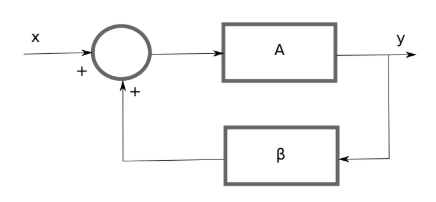
\includegraphics[width=0.5\textwidth]{marco-teorico/circuito-realimentado.png}
  \caption{Circuito realimentado.}
  \label{fig:circuito-realimentado}
\end{ilustracion}

Para el sistema de la ilustración \ref{fig:circuito-realimentado}, se tiene que la salida está dada por:

\begin{equation}
  y = A(x + y\beta)
\end{equation}

Donde:
\begin{itemize}
  \item $y$ es la salida del sistema
  \item $x$ es la entrada del sistema 
  \item $A$ es la ganancia del amplificador
  \item $\beta$ es el factor de realimentación
\end{itemize}

Por lo tanto, la ganancia del sistema realimentado está dada por:

\begin{equation}
  A_{fb} =\frac{y}{x} = \frac{A}{1-A\beta}
  \label{eq:ganancia-realimentacion}
\end{equation}

Cuando el resultado en el denominador es cero, entonces el sistema se encuentra en el límite de la estabilidad. Recordemos que un sistema con realimentación negativa es estable y el sistema con realimentación positiva es inestable \cite{herrera-osciladores}.

Para que un sistema oscile, debe cumplirse la condición de Barkhausen \cite{herrera-osciladores}:

\begin{equation}
  A(j\omega_o)\beta(j\omega_o) = 1
  \label{eq:condicion-barkhausen}
\end{equation}

Esta condición establece que para que exista oscilación, la ganancia de lazo debe ser unitaria a la frecuencia de oscilación $\omega_o$. Esto significa que:

\begin{itemize}
  \item La magnitud del producto $A\beta$ debe ser igual a 1
  \item El ángulo de fase del producto $A\beta$ debe ser 0° o un múltiplo entero de 360°
\end{itemize}

Por lo tanto,

\begin{equation}
  A(s)\beta(s) = 1 + 0j
  \label{eq:ganancia-oscilacion}
\end{equation}

donde

\begin{equation}
  \beta A = \frac{a_n s^n + a_{n-1} s^{n-1} + ... + a_o}{b_m s^m + b_{m-1} s^m + ... + b_o}
  \label{eq:ganancia-lazo}
\end{equation}

Sustituyendo $s = j\omega$, se puede deducir que los términos pares serían números reales y los términos impares serían imaginarios. Al agruparlos se puede simplificar en la siguiente ecuación.

\begin{equation}
  \beta A = \frac{N_p(s) + jN_i(s)}{D_p(s) + jD_i(s)}
  \label{eq:ganancia-lazo-simplificada}
\end{equation}

Donde $N_p(s)$ y $D_p(s)$ son los términos pares del numerador y denominador respectivamente, y $N_i(s)$ y $D_i(s)$ son los términos impares del numerador y denominador respectivamente.

Multiplicando numerador y denominador por el conjugado del denominador:

\begin{equation}
  \beta A = \frac{N_p(s) + jN_i(s)}{D_p(s) + jD_i(s)} \cdot \frac{D_p(s) - jD_i(s)}{D_p(s) - jD_i(s)}
  \label{eq:ganancia-lazo-conjugado}
\end{equation}

\begin{equation}
  \beta A = \frac{N_p(s)D_p(s) + N_i(s)D_i(s) + j(N_i(s)D_p(s) - N_p(s)D_i(s))}{D_p(s)^2 - D_i(s)^2}
  \label{eq:ganancia-lazo-final}
\end{equation}

de manera que igualando con la ecuación \ref{eq:ganancia-oscilacion} se tiene que:

\begin{equation}
  \begin{cases}
    \frac{N_p(s)D_p(s) + N_i(s)D_i(s)}{D_p(s)^2 - D_i(s)^2} = 1 \\
    \frac{N_i(s)D_p(s) - N_p(s)D_i(s)}{D_p(s)^2 - D_i(s)^2} = 0
  \end{cases}
  \label{eq:sistema-ecuaciones-oscilacion}
\end{equation}

resolviendo el sistema de ecuaciones \ref{eq:sistema-ecuaciones-oscilacion} se tiene que:

\begin{equation}
  \begin{cases}
    N_i = D_i \\
    N_p = D_p
  \end{cases}
\end{equation}

\subsection{Oscilador de puente de Wien}

Este circuito es uno de los osciladores más usados, por su sencillez y estabilidad \cite{herrera-osciladores}. Está realimentado negativamente por un circuito resistivo y positivamente por dos redes RC, en serie y paralelo.

\begin{ilustracion}[ht]
  \centering
  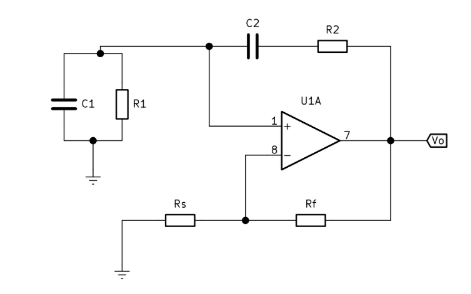
\includegraphics[width=0.5\textwidth]{marco-teorico/oscilador-wien.png}
  \caption{Oscilador de puente de Wien.}
  \label{fig:oscilador-wien}
\end{ilustracion}

Simplificando el circuito, tomando la ganancia del amplificador no inversor, resulta el circuito de la ilustración \ref{fig:oscilador-wien-simplificado}

\begin{ilustracion}[ht]
  \centering
  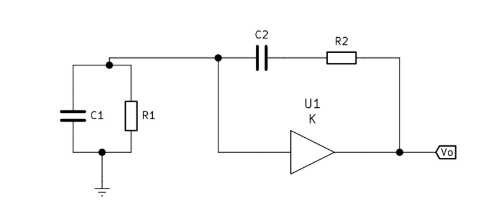
\includegraphics[width=0.5\textwidth]{marco-teorico/oscilador-wien-simplificado.png}
  \caption{Oscilador de puente de Wien simplificado.}
  \label{fig:oscilador-wien-simplificado}
\end{ilustracion}

con

\begin{equation}
  K = 1 + \frac{R_f}{R_s}
  \label{eq:ganancia-no-inversor}
\end{equation}

Ahora, utilizando el método del amplificador desvanecido para resolver el sistema,

\begin{equation}
  x_{31} = \frac{Z_p}{Z_p + Z_s}
\end{equation}

Donde, $Z_p= 1/sC_1 \parallel R_1$ y $Z_s=R_2 + sC_2$.

Por lo tanto, sustituyendo estos términos y simplificando la ecuación, se tiene:

\begin{equation}
  \beta A = A \frac{R1C2}{R1R2C1C2} \frac{s}{s^2 + s \frac{R2C2 + R1C1 + R1C2}{R1R2C1C2} + \frac{1}{R1R2C1C2}}
\end{equation}

Identificando los términos:

\begin{align}
  N_p(s) = 0 \\
  N_i(s) = A \frac{R1C2}{R1R2C1C2}s \\
  D_p(s) = s^2 + \frac{1}{R1R2C1C2} \\
  D_i(s) = s \left( \frac{R2C2 + R1C1 + R1C2}{R1R2C1C2} \right)
\end{align}

Partiendo de la igualdad $N_p = D_p$

\begin{equation}
  s^2 + \frac{1}{R1R2C1C2} = 0
\end{equation}

Se obtiene la frecuencia de oscilación del circuito,

\begin{equation}
  \omega_o = \pm \sqrt{\frac{1}{R1 \cdot R2 \cdot C1 \cdot C2}}
\end{equation}

Y de la igualdad $N_i = D_i$, se obtiene la ganancia del circuito

\begin{equation}
  A = \frac{R2 \cdot C2 + R1 \cdot C1 + R1 \cdot C2}{R1 \cdot C2}
\end{equation}

En la vida real, los variaciones de temperatura de los componentes dificulta mantener la estabilidad del puente de Wien \cite{herrera-osciladores}. Una manera de disminuir este efecto consiste en utilizar valores de resistencias iguales y de la misma tecnología, lo cual disminuye el efecto de oscilación debido a la temperatura.

Si $R_1 = R_2 = R$ y $C_1 = C_2 = C$, entonces la ganancia del circuito y su frecuencia de corte se vuelven:

\begin{equation}
  A = 3
  \label{eq:ganancia-oscilador-wien}
\end{equation}

\begin{equation}
  \omega_o = \frac{1}{RC}
  \label{eq:frecuancia-corte-oscilador-wien}
\end{equation}

\subsection{Controles de amplitud}

Para un oscilador, no es posible garantizar que mantenga las características
de oscilación durante toda su vida útil \cite{herrera-osciladores}.Para lograr esto, es necesario garantizar que la oscilación tenga un factor
de amortiguamiento no nulo, $A e^{\alpha t}sen(wt)$, de manera que pueda crecer y decrecer en amplitud.

Se desea entonces que en el arranque, ese factor $\alpha$ sea mayor que cero, y que crezca en magnitud hasta lograr niveles utilizables. Cuando esta señal sea grande, entonces el factor de amortiguamiento será menor que cero, evitando que el oscilador llegue a la zona no lineal \cite{herrera-osciladores}.